\section{Чисельні методи}

\subsection{Метод Монте-Карло}

Оскільки функція $f$, що дає зображення $t$ для даного набору параметрів $x$,
є складно влаштованою, вона не представлена в явному вигляді.
Інтегрування виразу, що містить цю функцію, не може бути проведено аналітично.
Метод Монте-Карло~---~чисельний метод, що підходить до розв'язку даної задачі.

Треба підрахувати інтеграл
\begin{equation}\label{eq:monte-carlo:source}
  q^* \left( t \right)
  = c_t
    \cdot \int\limits_{x \in X}
      x
      \cdot \exp{\left\{ - \frac{\left\| t - f\left( x \right) \right\|^2}
                                {2 \cdot \sigma^2_t}\right\}}
      \cdot \exp{\left\{ - \frac{\left\| x \right\|^2}{2} \right\}}
    d\,x,
\end{equation}
який є математичним сподіванням функції
стандартного ґаусового $n$-вимірного вектора
\begin{equation*}
  q^* \left( t \right)
  = c_t
    \cdot \Meanof{\xi}{
      \xi
      \cdot \exp{\left\{
          - \frac{\left\| t - f\left( \xi \right) \right\|^2}
                 {2 \cdot \sigma^2_t}
            \right\}}}, \qquad
    \xi_i \sim \mathcal{N}\left( 0, 1 \right).
\end{equation*}
Внесемо все в експоненту для полегшення машинних обчислень
\begin{equation*}
  q^* \left( t \right)
  = \Meanof{\xi}{
    \frac{\xi}{\left| \xi \right|}
    \cdot \exp{\left\{
        \ln{\left| \xi \right|}
        - \frac{\left\| t - f\left( \xi \right) \right\|^2}{2 \cdot \sigma^2_t}
        + \ln{c_t}
       \right\}
    }}.
\end{equation*}

Для отримання оцінки інтегралу
треба згенерувати $N$ векторів з $n$ незалежних випадкових величин,
що мають стандартний нормальний розподіл
\begin{equation*}
  \xi^{\left( i \right)}
  = \left\langle \xi^{\left( i \right)}_1, \xi^{\left( i \right)}_2, \dots,
  \xi^{\left( i \right)}_n \right\rangle,\qquad
  \xi^{\left( i \right)}_j \sim \mathcal{N}\left( 0, 1 \right).
\end{equation*}
Для кожного вектору розрахувати значення підінтегрального виразу
\begin{equation*}
  Q^{\left( i \right)}
  = \frac{\xi^{\left( i \right)}}{\left| \xi^{\left( i \right)} \right|}
  \cdot \exp{\left\{
      \ln{\left| \xi^{\left( i \right)} \right|}
      - \frac{\left\| t - f\left( \xi^{\left( i \right)} \right) \right\|^2}
             {2 \cdot \sigma^2_t}
      + \ln{c_t}
     \right\}
   }.
\end{equation*}
Значення константи $c_t$ визначимо з умови нормування
\begin{equation*}
  c_t \cdot
  \sum_{i=1}^{N}
    \exp{\left\{
      \frac{\left\| t - f\left( \xi^{\left( i \right)} \right) \right\|^2}
           {2 \cdot \sigma^2_t}
       + \frac{\left\| \xi^{\left( i \right)} \right\|^2}{2}
     \right\}}
  = 1.
\end{equation*}
Явний вигляд
\begin{equation*}
  c_t
  = \frac{1}{\sum\limits_{i=1}^{N}
    \exp{\left\{
      \frac{\left\| t - f\left( \xi^{\left( i \right)} \right) \right\|^2}
           {2 \cdot \sigma^2_t}
      + \frac{\left\| \xi^{\left( i \right)} \right\|^2}{2}
    \right\}}}.
\end{equation*}
Оцінкою інтегралу буде середнє значення
\begin{equation*}
  \overline{Q}_N = \frac{\sum\limits_{i=1}^{N}
    \hat{Q}^{\left( i \right)}}{N}.
\end{equation*}

Визначимо оптимальне значення $N$.
Згадаємо центральну граничну теорему
\begin{equation*}
  \sqrt{N}
    \cdot \frac{\overline{Q}_N - M\left( Q \right)}
    {\sqrt{D\left( Q \right)}} \Rightarrow \mathcal{N}\left( 0, 1 \right).
\end{equation*}
Для певного $z_{\gamma} > 0$
\begin{equation*}
  \mathbb{P}\left(
    \sqrt{N}
    \cdot \frac{\overline{Q}_N - M\left( Q \right)}{\sqrt{D\left( Q \right)}}
    \le z_{\gamma}
  \right) = \Phi\left( z_{\gamma} \right),
\end{equation*}
де $\Phi$~---~інтегральна функція стандартного ґаусового розподілу.
Нас цікавить ймовірність
\begin{equation*}
  \mathbb{P}\left(
    -z_{\gamma} \le
    \sqrt{N}
    \cdot \frac{\overline{Q}_N - M\left( Q \right)}{\sqrt{D\left( Q \right)}}
    \le z_{\gamma}
  \right)
  = \Phi\left( z_{\gamma} \right) - \Phi\left( -z_{\gamma} \right).
\end{equation*}
Використаємо модуль для перевірки входження виразу в довірчий інтервал
та скористаємося симетричністю ґаусового розподілу
\begin{equation*}
  \mathbb{P}\left(
    \left|
      \sqrt{N}
      \cdot \frac{\overline{Q}_N - M\left( Q \right)}{\sqrt{D\left( Q \right)}}
    \right|
    \le z_{\gamma}
  \right)
  = 2 \cdot \Phi\left( z_{\gamma} \right) - 1.
\end{equation*}
Поділимо обидві частини нерівності на модуль середнього значення виборки
\begin{equation*}
  \mathbb{P}\left(
    \left|
      \sqrt{N}
      \cdot \frac{\overline{Q}_N - M\left( Q \right)}
        {\overline{Q}_N \cdot \sqrt{D\left( Q \right)}}
    \right|
    \le \frac{z_{\gamma}}{\left| \overline{Q}_N \right|}
  \right)
  = 2 \cdot \Phi\left( z_{\gamma} \right) - 1.
\end{equation*}
Позначимо відносну похибку
\begin{equation*}
  \varepsilon
  = \left| \frac{\overline{Q}_N - M\left( Q \right)}{\overline{Q}_N} \right|
\end{equation*}
та перепишемо вираз
\begin{equation*}
  \mathbb{P}\left(
    \left|
      \sqrt{N}
      \cdot \frac{\varepsilon}
        {\sqrt{D\left( Q \right)}}
    \right|
    \le \frac{z_{\gamma}}{\left| \overline{Q}_N \right|}
  \right)
  = 2 \cdot \Phi\left( z_{\gamma} \right) - 1.
\end{equation*}
Перенесемо все окрім кореню від кількості спроб в праву частину нерівності
\begin{equation*}
  \mathbb{P}\left(
    \left|
      \sqrt{N}
    \right|
    \le \left|
      \frac{z_{\gamma} \cdot \sqrt{D\left( Q \right)}}
      {\varepsilon \cdot \overline{Q}_N} \right|
  \right)
  = 2 \cdot \Phi\left( z_{\gamma} \right) - 1
\end{equation*}
та піднесемо обидві частини нерівності до квадрату
\begin{equation*}
  \mathbb{P}\left(
    N
    \le \frac{z^2_{\gamma} \cdot D\left( Q \right)}
      {\varepsilon^2 \cdot \overline{Q}_N^2}
  \right)
  = 2 \cdot \Phi\left( z_{\gamma} \right) - 1.
\end{equation*}
Перепозначимо отриману ймовірність
\begin{equation*}
  \mathbb{P}\left(
    N
    \le \frac{z^2_{\gamma} \cdot D\left( Q \right)}
      {\varepsilon^2 \cdot \overline{Q}_N^2}
  \right)
  = \gamma.
\end{equation*}
Щоб виразити $z_{\gamma}$,
потрібно скористатися квантилєм нормального розподілу
\begin{equation*}
  \Phi^{-1}\left( \frac{\gamma + 1}{2} \right) = z_{\gamma}.
\end{equation*}
Щоб відносна похибка обчислення математичного сподівання методом Монте-Карло
не перевищувала $\varepsilon$ з ймовірністю $\gamma$ і вище,
необхідна та достатня кількість ітерацій рахується за формулою
\begin{equation}\label{eq:mc-iterations}
    N
    = \left\lceil \frac{z^2_{\gamma} \cdot D\left( Q \right)}
      {\varepsilon^2 \cdot \overline{Q}_N^2} \right\rceil, \qquad
    z_{\gamma} = \Phi^{-1}\left( \frac{\gamma + 1}{2} \right).
\end{equation}
Коли дисперсія отриманої випадкової величини $Q$ невідома,
використовується її незміщена оцінка
\begin{equation*}
  \widetilde{Q}_N
  = \frac{
    \sum\limits_{i=1}^{N}
      \left( \hat{Q}^{\left( i \right)}\left( x \right) \right)^2
    - \overline{Q}_N^2}{N - 1}.
\end{equation*}

Формула \eqref{eq:mc-iterations} використовується лише для перевірки того,
чи дає наявна вибірка з $N$ елементів відповідь з вказаною похибкою.
Спочатку необхідно дати алгоритму ``розігрітись'' і не порівнювати значення $N$
з необхідною кількістю кроків.
Також немає необхідності у перевірці відповідності значення $N$
на кожній ітерації,
особливо якщо це займає багато часу ---
достатньо робити перерахунок кожні $100$ або $1000$ кроки в залежності від
інтегралу.

\subsection{Мінімізація цільової функції}

При мінімізації цільової функції \eqref{eq:minimize}
виникає кілька складностей:
\begin{enumerate}
  \item наявність локальних мінімумів;
  \item складний аналітичний вираз функції визуалізації;
  \item недиференційованість.
\end{enumerate}

Останній пункт може викликати сумніви,
тому переглянемо причини його справедливості.
Множина пікселів дискретна за умовою, а опорні точки прив'зані до неї.
Множина можливих кольорів дискретна за технічними особливостями
комп'ютерної техніки, тому будь-яка зміна кольору відбувається дискретно.
Алгоритми екранного згладжування межі моделі зроблено для того,
щоб межа полігонів була трохи розмитою.
При недостатньому згладжуванні цю межу явно видно
(рис. \ref{fig:calculation:smoothing-issue}),
що дає різкий стрибок цільової функції,
коли модель починає (перестає) обіймати нові (старі) пікселі,
через специфіку відображення діагональних ліній.

\begin{figure}[h]
  \centering
  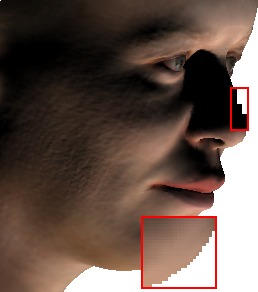
\includegraphics[width=0.75\textwidth]{images/face-unsmoothed.png}
  \caption{Візуалізація обличчя зі збільшеними діагональними лініями}
  \label{fig:calculation:smoothing-issue}
\end{figure}

Функція візуалізації є складною, бо
\begin{enumerate}
  \item
    треба визначити невидимі вершини;
  \item
    проводиться фільтрація,
    згладжування та інші процедури покращення зображення;
  \item
    розрахунок самозатінення містить функцію візуалізації,
    проте без тіней та текстури.
\end{enumerate}

Для запобігання локальних мінімумів
використовують координати знайдених опорних точок обличчя.

Диференціювати цільову функцію можна чисельними методами з таким $dx$,
при якому стрибки не будуть суттєвими.

Щоб диференціювати цільову функцію аналітично,
автори попередніх робіт один раз на певну кількість ітерацій
(наприклад, $1000$)
шукають видимі вершини/трикутники та розраховують самозатінення на них.
Далі з'являється можливість розрахувати похідні аналітично
і використовувати у методах, що потребують якобіан
(градіентний спуск, метод Ньютона-Ґауса тощо).
